\documentclass{article}
\usepackage[utf8]{inputenc}


\title{Common activation functions used in neural net}
\author{}
\date{}

\usepackage{natbib}
\usepackage{graphicx}
\usepackage{amsmath,amssymb}
\usepackage[left=2.5cm,right=2.5cm,top=1cm,bottom=1.25cm]{geometry}
\usepackage{hyperref}
\usepackage{multicol}
\usepackage[export]{adjustbox}
\usepackage{sidecap}
\hypersetup{colorlinks=true,urlcolor=blue}
\renewcommand{\thesubsection}{\arabic{subsection}.}


\begin{document}

\maketitle

\section*{Activation function}
The activation function of a node in an artificial neural network converts an input signal to an output signal. This is loosely based on the biological neuron where the activation function decides whether or not to pass the signal accumulated in a cell body to the next cell.


\section*{Why we need activation functions}

\begin{itemize}
    \item Activation functions determine the firing potential of a neuron and can act as a decision function(i.e., whether the neuron should fire or not).
    \item  A feedforward neural network with linear activation and any number of hidden layers is equivalent to just a linear neural neural network with no hidden layer. For example lets consider the neural network in figure with two hidden layers and no activation:\\
    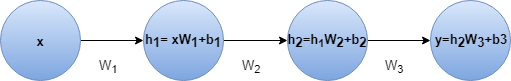
\includegraphics[scale=0.75, center]{neural_net_three_layers.png}
    \begin{align*}
        y &= h_2 W_3 + b_3 \\
          &= (h_1 W_2 + b_2) W_3 + b_3 \\
          &= h_1 W_2 W_3 + b_2 W_3 + b_3 \\
          &= (x W_1 + b_1) W_2 W_3 + b_2 W_3 + b_3 \\
          &= x W_1 W_2 W_3 + b_1 W_2 W_3 + b_2 W_3 + b_3 \\
          &= x W' + b'
    \end{align*}
    So we could replace this neural net with a single layer neural net.This can be extended to $n$ layers. This indicates adding layers doesn't increase the approximation power of a linear neural net at all. We need non-linear activation functions to approximate non-linear functions and most real world problems are highly complex and non-linear. In fact when the activation function is non-linear, then a two-layer neural network with sufficiently large number of hidden units can be proven to be a universal function approximator.
    \item Activation functions are also needed for squashing the unbounded linearly weighted sum from neurons.
\end{itemize}

\section*{Some desirable properties of activation functions}
\begin{itemize}
    \item \textit{Nonlinear:} To approximate complex non-linear functions the activation function also needs to be non-linear.
    \item \textit{Continuously differentiable:} This is desirable for gradient based optimization methods.
    \item \textit{Monotonic:} When the activation function is monotonic, the error surface associated with a single-layer model is guaranteed to be convex.
    \item \textit{Approximates Identity function($f(x)=x$) near origin:} When activation functions have this property, the neural network will learn efficiently when its weights are initialized with small random values. This is because gradient near origin will be close to $1$. When the activation function does not approximate identity near the origin, special care must be used when initializing the weights. Activation functions where $f(0)=0$, $f'(0)=1$ and $f'(x)$ is continuous at $0$ have this property.  
    \item \textit{Range:} When the range of activation function is finite, gradient-based training methods tend to be more stable because only limited range of values affect gradient significantly. When the range is infinite, training is generally more efficient(faster) because most of the values contribute significantly to gradients. In the latter case, smaller learning rates are typically necessary.  
    
\end{itemize}

\section*{Common activation functions}

\subsection{Sigmoid}
\begin{itemize}
    \item Equation: $f(x) = \sigma(x) = \frac{1}{1+e^{-x}}$
    \item Derivative: $f'(x) = \sigma(x) (1 - \sigma(x))$
    \item Graph:\\ 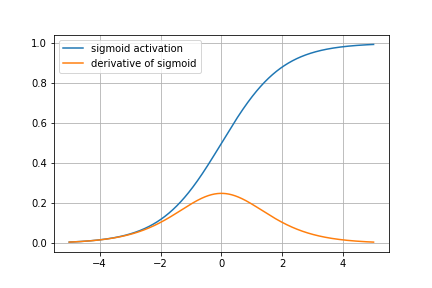
\includegraphics[ center]{sigmoid.png}
    \item Pros
    \begin{enumerate}
        \item Its non-linear, continuously differentiable, monotonic.
        \item Output is in the range of $[0, 1]$ so it can be used as a binary classifier or estimate probability.
        \item The bounded output means the activations won't blow up.
    \end{enumerate}
    \item Cons
    \begin{enumerate}
        \item Towards either end of the sigmoid function the change in activation is very small as input is changed and gradient is very close to zero. This gives rise to the \textbf{vanishing gradients problem}. This means that neurons in those regions will get very little gradient update and become saturated. The learning will become very slow.
        \item Sigmoid outputs are not zero centered and it does not approximate identity function near origin.
        \item Exponential function is computationally expensive.
    \end{enumerate}
\end{itemize}

\subsection{Tanh}
\begin{itemize}
    \item Equation: $f(x) = \tanh(x) = \frac{e^x-e^{-x}}{e^x+e^{-x}}$
    \item Derivative: $f'(x) = 1 - f(x)^2$
    \item Graph:\\ 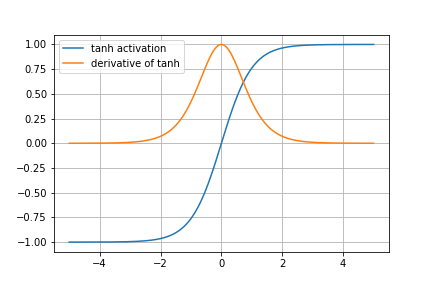
\includegraphics[ center]{tanh.png}
    \item Pros
    \begin{enumerate}
        \item Its non-linear, continuously differentiable, monotonic.
        \item Output is bounded in the range of $[-1, +1]$ so the activation won't blow up.
        \item It approximates identity function near origin. Optimization is easier than sigmoid because gradient is steeper.
    \end{enumerate}
    \item Cons
    \begin{enumerate}
        \item Suffers vanishing gradients problem just like sigmoid. 
        \item Also computationally expensive.
    \end{enumerate}
\end{itemize}

\subsection{ReLU(Rectified Linear Unit)}
\begin{itemize}
    \item Equation: 
    \begin{equation*}
        f(x)=\begin{cases}
        x, & \text{$x>=0$}.\\
        0, & \text{$x<0$}.
        \end{cases}
    \end{equation*}
    \item Derivative:
    \begin{equation*}
        f'(x)=\begin{cases}
        1, & \text{$x>=0$}.\\
        0, & \text{$x<0$}.
        \end{cases}
    \end{equation*}
    \item Graph:\\ 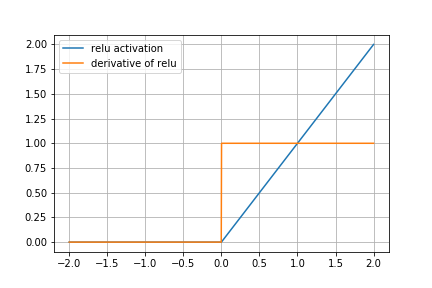
\includegraphics[ center]{relu.png}
    \item Pros
    \begin{enumerate}
        \item Its non-linear, monotonic.
        \item The gradient does not saturate like sigmoid or tanh so it rectifies the vanishing gradient problem. 
        \item The second derivative of the rectifying operation is $0$ almost everywhere, and the derivative of the rectifying operation is $1$ everywhere that the unit is active. This means that the gradient direction is far more useful for learning than it would be with activation functions that introduce second-order effects(sigmoid and tanh).
        \item It is computationally inexpensive.
    \end{enumerate}
    \item Cons
    \begin{enumerate}
        \item When the activation is zero for a neuron it doesn't get any further update via gradient descent. So such neuron will stop responding to variations in error or input signal.This is called \textbf{dying relu problem}. When initializing the parameters of the network, it can be a good practice to set all elements of bias to a small, positive value, such as $0.1$. This makes it very likely that the rectified linear units will be initially active for most inputs in the training set and allow the derivatives to pass through.
        \item It cannot be used in the output layer of a network. We usually use sigmoid(binary) or softmax(multiclass) for classification task and linear function for regression task.
        \item The range of relu is $[0, \infty)$. This means it can blow up the activation.
        \item ReLU is not differentiable at $x=0$. However it sill works for gradient based learning in practice because neural training training algorithms do not usually arrive at a local minimum of the cost function, but instead merely reduce its value significantly and gradient based optimization on a digital computer is subject to numerical error anyway.  
    \end{enumerate}
\end{itemize}

\subsection{Leaky ReLU and Parametric ReLU}
\begin{itemize}
    \item Equation: 
    \begin{equation*}
        f(x)=\begin{cases}
        x, & \text{$x>=0$}.\\
        \alpha x, & \text{$x<0$}.
        \end{cases}
    \end{equation*}
    $\alpha=0.01$ for Leaky ReLU
    \item Derivative:
    \begin{equation*}
        f'(x)=\begin{cases}
        1, & \text{$x>=0$}.\\
        \alpha, & \text{$x<0$}.
        \end{cases}
    \end{equation*}
    \item Graph:\\ 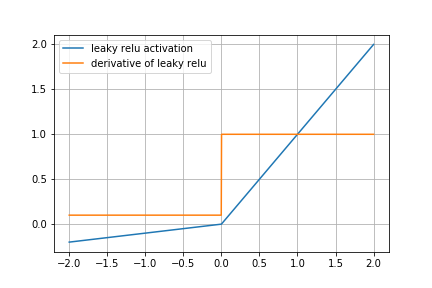
\includegraphics[center]{leaky_relu.png}
    \item Pros
    \begin{enumerate}
        \item It has non-zero slope everywhere and so doesn't have the dying relu problem.
    \end{enumerate}
    \item Cons
    \begin{enumerate}
        \item The result is not always consistent and in practice doesn't always perform better than plain relu.
    \end{enumerate}
\end{itemize}

\subsection{ELU(Exponential Linear Unit)}
\begin{itemize}
    \item Equation: 
    \begin{equation*}
        f(x)=\begin{cases}
        x, & \text{$x>0$}.\\
        \alpha (e^x-1), & \text{$x<=0$}.
        \end{cases}
    \end{equation*}
    \item Derivative:
    \begin{equation*}
        f'(x)=\begin{cases}
        1, & \text{$x>=0$}.\\
        \alpha e^x, & \text{$x<0$}.
        \end{cases}
    \end{equation*}
    \item Graph:\\ 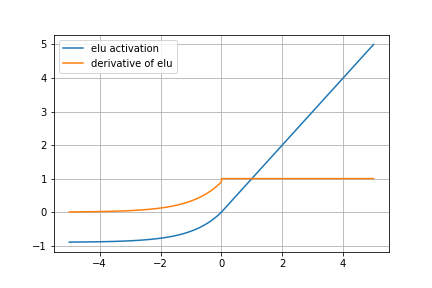
\includegraphics[center]{elu.png}
    \item Pros
    \begin{enumerate}
        \item It doesn't have dying relu problems.
        \item It becomes smooth slowly for negative inputs unlike relu which sharply becomes smooth.
    \end{enumerate}
    \item Cons
    \begin{enumerate}
        \item Output becomes saturated for large negative values and gradient becomes zero for neurons in that region.
    \end{enumerate}
\end{itemize}


\end{document}
